\documentclass{article}
\usepackage{tikz}
\usepackage{amsmath}
\usepackage{bm}
\usepackage{scalerel}
\usepackage{pgfplots}
\usepackage{mathpazo}
\pgfplotsset{width=7cm,compat=1.8}
\usetikzlibrary{patterns}
\usetikzlibrary{arrows,shapes,calc}
\usetikzlibrary{external}
\tikzset{external/system call={pdflatex \tikzexternalcheckshellescape -halt-on-error
        -interaction=batchmode -jobname "\image" "\texsource" && %  or ;
pdftops -eps "\image".pdf}}
\tikzexternalize


\begin{document}
 \hspace{-3cm}
 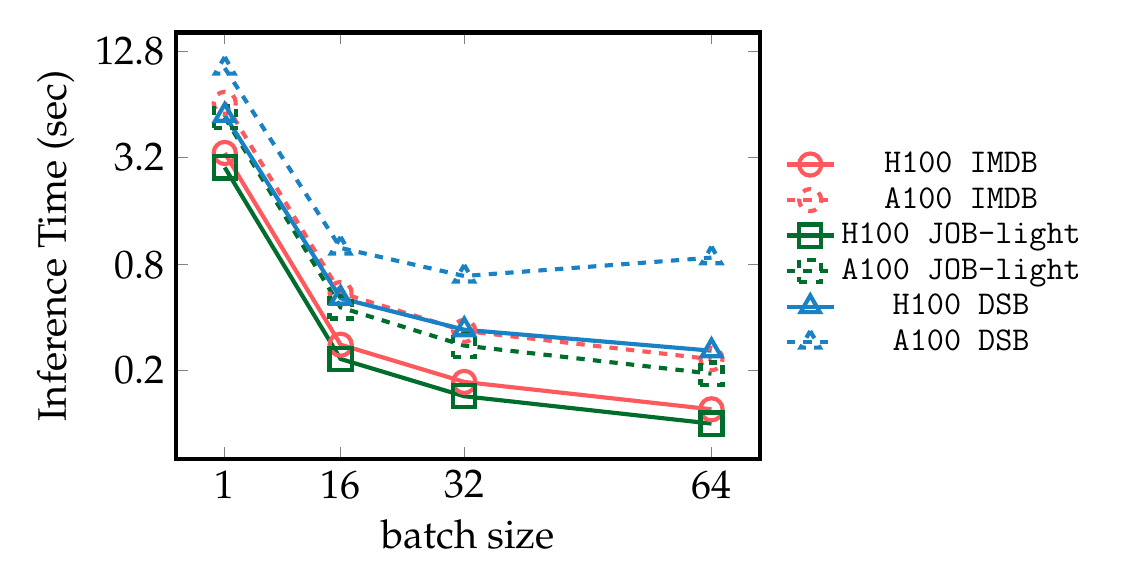
\begin{tikzpicture}
 \tikzstyle{every node}=[font=\large]
 \definecolor{uc}{HTML}{ff595e}
 \definecolor{ic}{HTML}{006d2c}
 \definecolor{uic}{HTML}{1982c4}
 \centering
 \begin{axis}[
 height=7cm, width=9cm,
 line width= 1.5pt,
 %enlarge y limits={value=.1,upper},
 % ymin=-1.3010, ymax=1.3010,
  % ymin=0, ymax=1.00,
 %ymode=log,
 %log origin=infty,
 enlarge x limits=true,
 legend style={
  draw=none,
  at={(1.3, 0.75)},
  anchor=north,
  legend columns=1,
  /tikz/every even column/.append style={column sep=0.6cm}
 },
 ylabel={Inference Time (sec)},
% ['-1.00', '-0.70', '-0.40', '-0.10', '0.20', '0.51', '0.81', '1.11']
 ytick={-0.7, -0.10, 0.51, 1.11},
 yticklabels={0.2, 0.8, 3.2, 12.8},
 xmin=1, xmax = 64,
 xlabel={batch size},
 xtick={1, 16, 32, 64},
 xticklabels={1, 16, 32, 64},
    label style={font=\Large},
    tick label style={font=\Large}
 %xlabel={Number of Stacking Blocks},
 %symbolic x coords={
 % Facebook, Gowalla, WikiConflict, Google, DBLP, Berkstan, Youtube, Petster, Flickr,
 %Indochina },
 %xtick=data,
 ]

   
%IMDB H100
\addplot [color=uc, mark=o, mark size=4pt] 
coordinates {
    (1, 0.533)
    (16, -0.553)
    (32, -0.764)
    (64, -0.919)
};


% IMDB A100
  \addplot [color=uc,mark=o, mark size=4pt, dashed] 
  coordinates {
(1, 0.817)
(16, -0.260)
(32, -0.475)
(64, -0.635)
      };

%Job-light H100
  \addplot [color=ic,mark=square, mark size=4pt] coordinates {
(1, 0.451)
(16, -0.634)
(32, -0.845)
(64, -1.000)
 };
 
 
%Job-light A100
  \addplot [color=ic,mark=square, mark size=4pt, dashed] 
  coordinates {
(1, 0.735)
(16, -0.342)
(32, -0.558)
(64, -0.717)
 };
 

    
%DSB H100
  \addplot [color=uic,mark=triangle, mark size=4pt] coordinates {
(1, 0.747)
(16, -0.290)
(32, -0.468)
(64, -0.587)
    };





%DSB A100
  \addplot [color=uic,mark=triangle, mark size=4pt, dashed] coordinates {
(1, 1.014)
(16, -0.005)
(32, -0.164)
(64, -0.060)
    };
    
    \legend{
        {\large $\texttt{H100 IMDB}$}, 
        {\large $\texttt{A100 IMDB}$},
        {\large $\texttt{H100 JOB-light}$}, 
        {\large $\texttt{A100 JOB-light}$}, 
        {\large $\texttt{H100 DSB}$}, 
        {\large $\texttt{A100 DSB}$}
        }
 \end{axis}
 \end{tikzpicture}
\end{document}